\chapter{Diagramas}

En este apartado se encuentran las representaciones visuales que definen la estructura y el comportamiento del sistema. Se incluyen diagramas de casos de uso, que identifican las interacciones entre actores y funcionalidades, y diagramas de secuencia, que detallan el intercambio de mensajes durante la ejecución de tareas concretas.

\section{Casos de uso}

El diagrama general de casos de uso se encuentra en la documentación original del proyecto. Los actores contemplados son el usuario visitante, el usuario registrado, la empresa y el administrador; las funcionalidades son las descritas en la sección de casos de uso.

\section{Secuencia}

\begin{figure}[htbp]
  \centering
  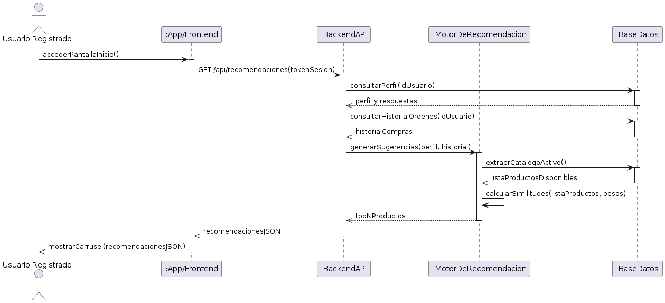
\includegraphics[width=\textwidth,keepaspectratio]{diagrama-cu02.png}
  \caption{Diagrama de secuencia del CU02}
\end{figure}

\begin{figure}[htbp]
  \centering
  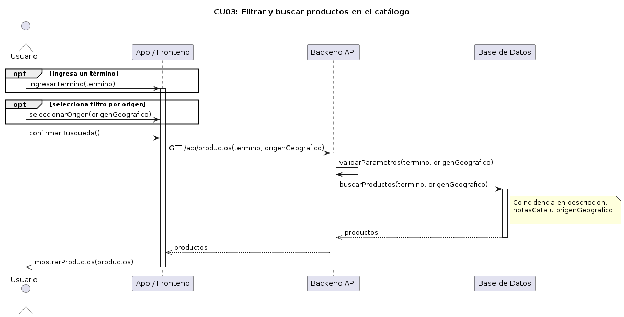
\includegraphics[width=\textwidth,keepaspectratio]{diagrama-cu03.png}
  \caption{Diagrama de secuencia del CU03}
\end{figure}

\begin{figure}[htbp]
  \centering
  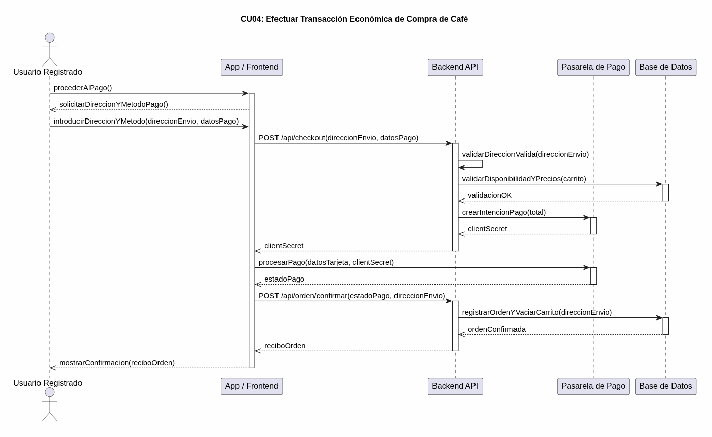
\includegraphics[width=\textwidth,keepaspectratio]{diagrama-cu04.png}
  \caption{Diagrama de secuencia del CU04}
\end{figure}

\begin{figure}[htbp]
  \centering
  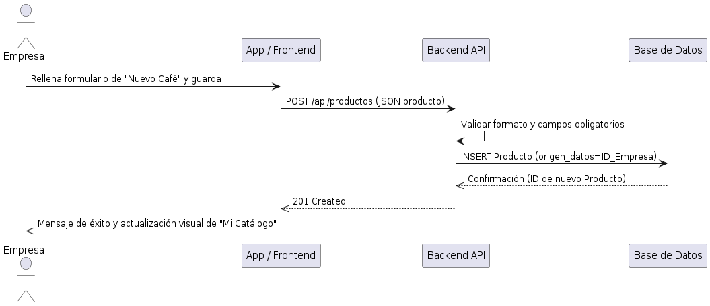
\includegraphics[width=\textwidth,keepaspectratio]{diagrama-cu05.png}
  \caption{Diagrama de secuencia del CU05}
\end{figure}
